\section{Website kết quả và khả năng tái lập}
\label{sec:website}

\subsection{Mục tiêu và địa chỉ công khai}

Báo cáo không chỉ trình bày kết quả trong tệp PDF mà còn công bố một website tĩnh để
người đọc có thể kiểm tra dữ liệu, biểu đồ và dự báo một cách trực quan. Website có
địa chỉ:

\begin{center}
\url{https://huyduong5.github.io/colorado-river-flow-atlas/}
\end{center}

Mã nguồn công khai nằm tại:

\begin{center}
\url{https://github.com/huyduong5/colorado-river-flow-atlas}
\end{center}

Website được thiết kế để trả lời ba câu hỏi: dữ liệu trông như thế nào; các phát hiện
chính về xu hướng, mùa vụ và cực trị ra sao; mô hình dự báo hoạt động thế nào. Mỗi
trang đều có liên kết đến dữ liệu gốc hoặc tệp kết quả tương ứng, để người đọc không
phải tin vào hình ảnh mà không có nguồn.

\begin{figure}[H]
\centering
\begin{minipage}{0.31\linewidth}
\centering

\includegraphics[width=\linewidth]{qr_website.png}
\end{minipage}
\hfill
\begin{minipage}{0.31\linewidth}
\centering

\includegraphics[width=\linewidth]{qr_github.png}
\end{minipage}
\caption{Mã QR đến website kết quả (trái) và kho mã nguồn (phải).}
\label{fig:qr}
\end{figure}

\subsection{Kiến trúc website}

Website là một ứng dụng React viết bằng TypeScript, được đóng gói bằng Vite. Dữ liệu
không được nhúng trực tiếp vào mã nguồn mà được đọc từ các tệp JSON/CSV trong
\texttt{public/data}. Cách tách dữ liệu khỏi giao diện giúp website có thể cập nhật
kết quả mà không phải sửa component. Các biểu đồ dùng ECharts; bảng và thẻ số liệu
dùng component React thuần.

Cấu trúc chính:

\begin{itemize}[leftmargin=1.4em]
  \item \texttt{code/src/colorado\_flow/export\_web.py}: sinh dữ liệu JSON cho
  website từ kết quả pipeline.
  \item \texttt{code/web/public/data/}: dữ liệu đã xuất, gồm manifest, chuỗi thời
  gian, sự kiện cực trị, dự báo và chỉ số mô hình.
  \item \texttt{code/web/src/pages/}: tám trang giao diện.
  \item \texttt{code/web/src/components/}: layout, biểu đồ, bảng, thẻ số liệu và
  thành phần điều hướng.
  \item \texttt{.github/workflows/deploy-pages.yml}: build và triển khai lên GitHub
  Pages mỗi khi push lên nhánh \texttt{main}.
\end{itemize}

Vite được cấu hình với \texttt{base: './'} để các tệp tĩnh hoạt động đúng khi website
được phục vụ từ thư mục con của GitHub Pages. Điều hướng dùng hash routing, nhờ đó
việc tải lại một trang con không tạo yêu cầu 404 trên máy chủ tĩnh. Đây là những
chi tiết kỹ thuật nhỏ nhưng quan trọng để website công khai hoạt động ổn định.

\subsection{Các trang và nội dung}

Bảng~\ref{tab:website-pages} liệt kê tám trang. Mỗi trang có một mục tiêu riêng,
tránh lặp lại cùng một biểu đồ ở nhiều nơi.

\begin{table}[H]
\centering
\small
\begin{tabularx}{\linewidth}{@{}lX@{}}
\toprule
\textbf{Trang} & \textbf{Nội dung chính} \\
\midrule
Tổng quan & Thẻ KPI, tóm tắt phát hiện, liên kết nhanh đến các phần. \\
Khám phá dữ liệu & Chuỗi thời gian, phân bố, thống kê mô tả, bảng dữ liệu. \\
Xu hướng \& mùa vụ & Trung bình theo tháng/năm, STL, ACF, nhận xét. \\
Cực trị Q95 & Ngưỡng, số ngày, số đợt, bảng sự kiện, bản đồ nhiệt. \\
Dự báo 7 ngày & Dự báo rolling-origin, bảng chỉ số theo horizon. \\
So sánh mô hình & RMSE/MAE/NSE, so sánh Naive, Seasonal và LightGBM. \\
Phương pháp & Pipeline, split, đặc trưng, tham số, giới hạn. \\
Tải về & PDF, source ZIP, dữ liệu CSV, manifest và checksum. \\
\bottomrule
\end{tabularx}
\caption{Các trang chính của website kết quả.}
\label{tab:website-pages}
\end{table}

\begin{figure}[H]
\centering
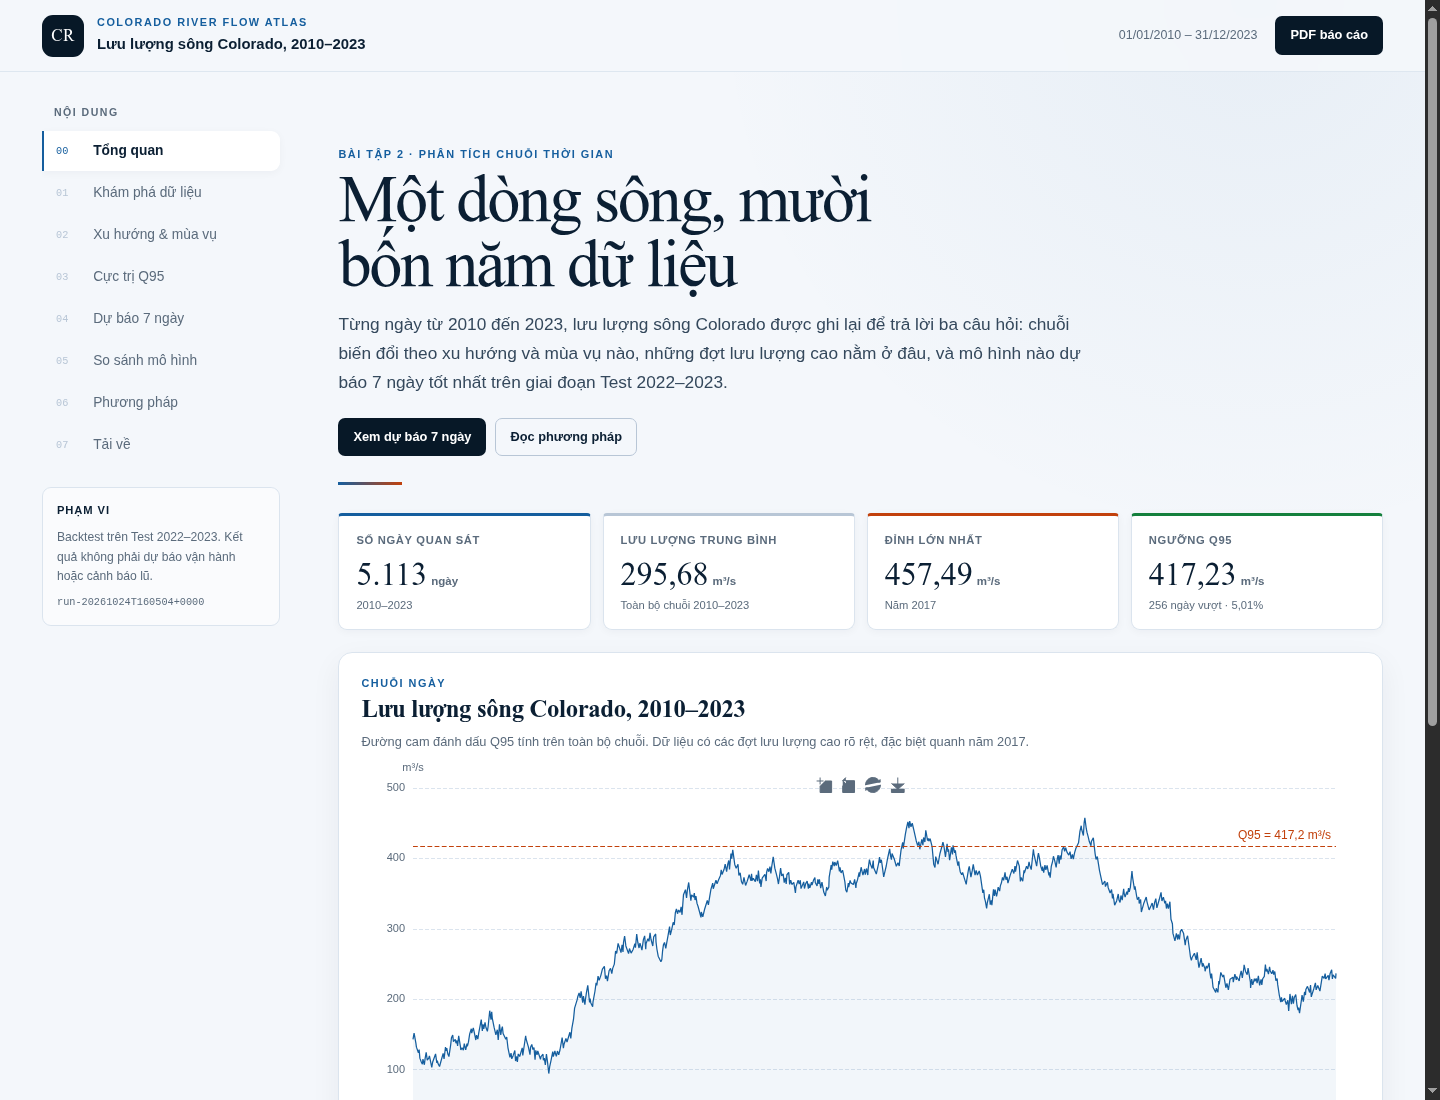
\includegraphics[width=0.82\linewidth]{website_overview.png}
\caption{Trang Tổng quan với các thẻ KPI và tóm tắt phát hiện.}
\label{fig:website-overview}
\end{figure}

Hình~\ref{fig:website-overview} cho thấy trang Tổng quan đặt các con số quan trọng ở
vị trí dễ thấy: số ngày, lưu lượng trung bình, ngưỡng Q95, số đợt và kết quả mô hình.
Các thẻ này được sinh từ cùng một manifest với báo cáo, nên nếu pipeline chạy lại,
website và báo cáo cùng thay đổi.

\subsection{Trang dự báo và tương tác}

Trang Dự báo cho phép chọn horizon và xem chuỗi dự báo so với quan trắc. Hình
\ref{fig:website-forecast} là ảnh chụp trang này ở kích thước desktop. Biểu đồ chính
hiển thị dự báo rolling-origin; bảng bên dưới tóm tắt RMSE, MAE và NSE theo horizon.
Người đọc có thể đối chiếu với Bảng~\ref{tab:metrics-horizon} trong báo cáo.

\begin{figure}[H]
\centering
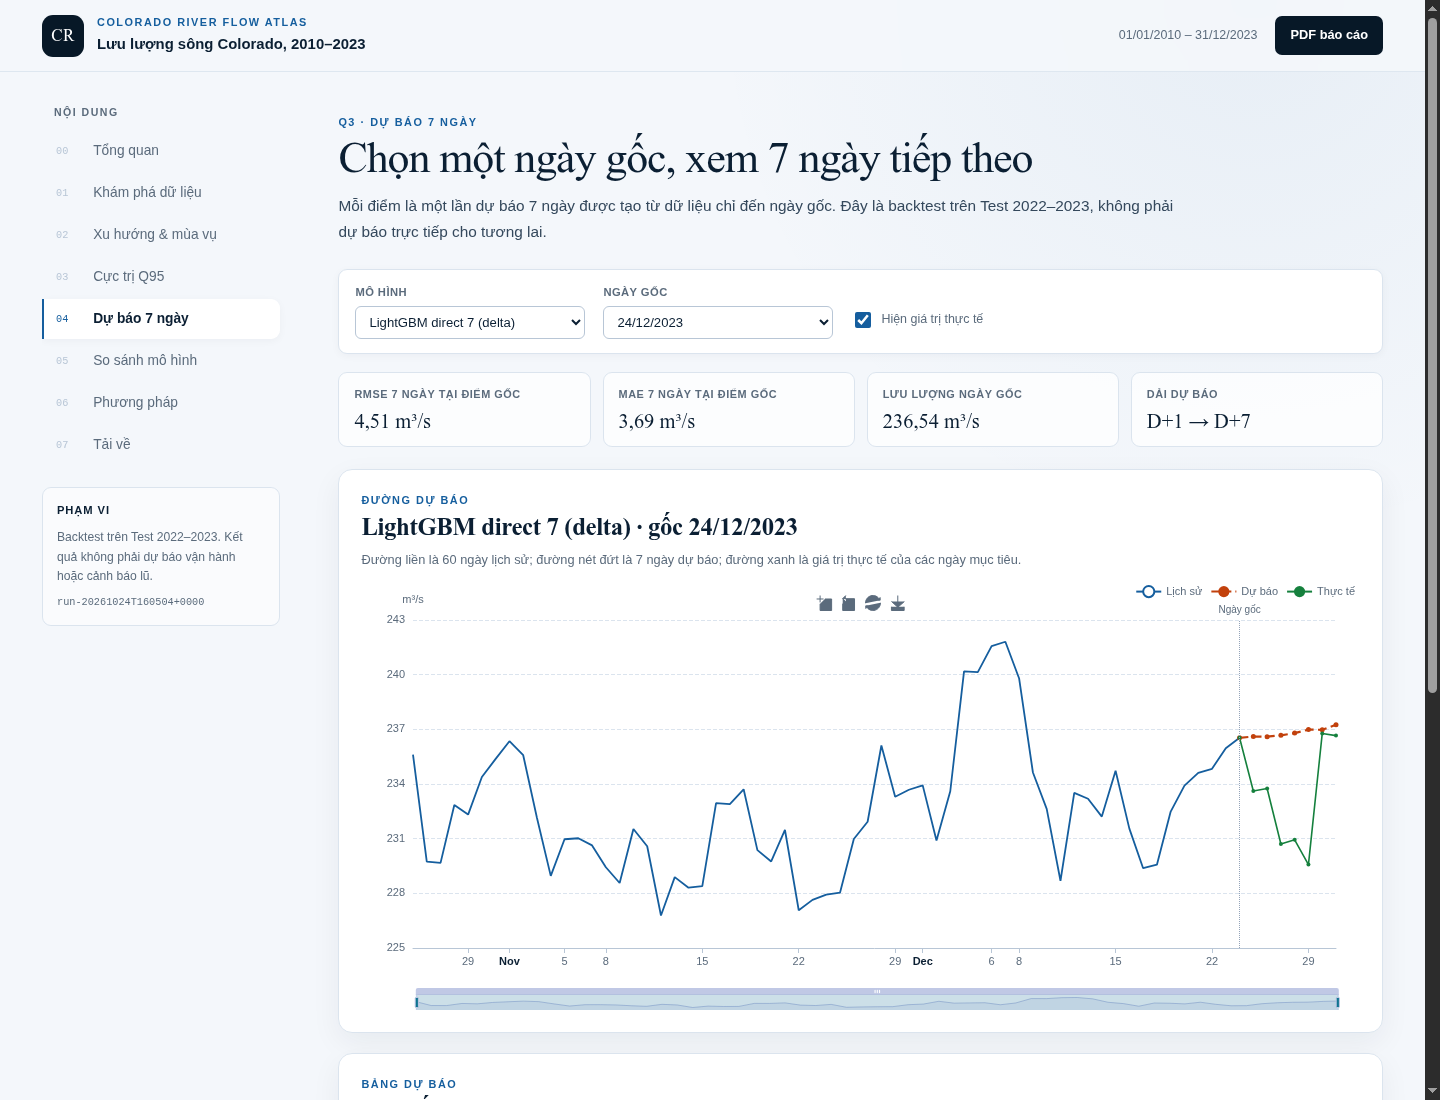
\includegraphics[width=0.94\linewidth]{website_forecast.png}
\caption{Trang Dự báo 7 ngày với biểu đồ rolling-origin và bảng chỉ số.}
\label{fig:website-forecast}
\end{figure}

Website không chạy mô hình trong trình duyệt. Mọi dự báo được tính sẵn trong pipeline
và lưu thành tệp JSON. Cách làm này giữ website nhẹ, không cần backend và bảo đảm
rằng người đọc nhìn thấy đúng kết quả đã được đánh giá, không phải một lần chạy mô
hình ngẫu nhiên khác. Đổi lại, website không thể nhận dữ liệu mới theo thời gian thực;
muốn cập nhật phải chạy lại pipeline và deploy.

\subsection{Trang tải về và tính minh bạch}

Trang Tải về cung cấp báo cáo PDF, mã nguồn, dữ liệu đã xử lý và manifest. Mỗi tệp
có tên rõ ràng và kèm checksum trong \texttt{SHA256SUMS}. Hình
\ref{fig:website-downloads} là ảnh chụp trang này.

\begin{figure}[H]
\centering
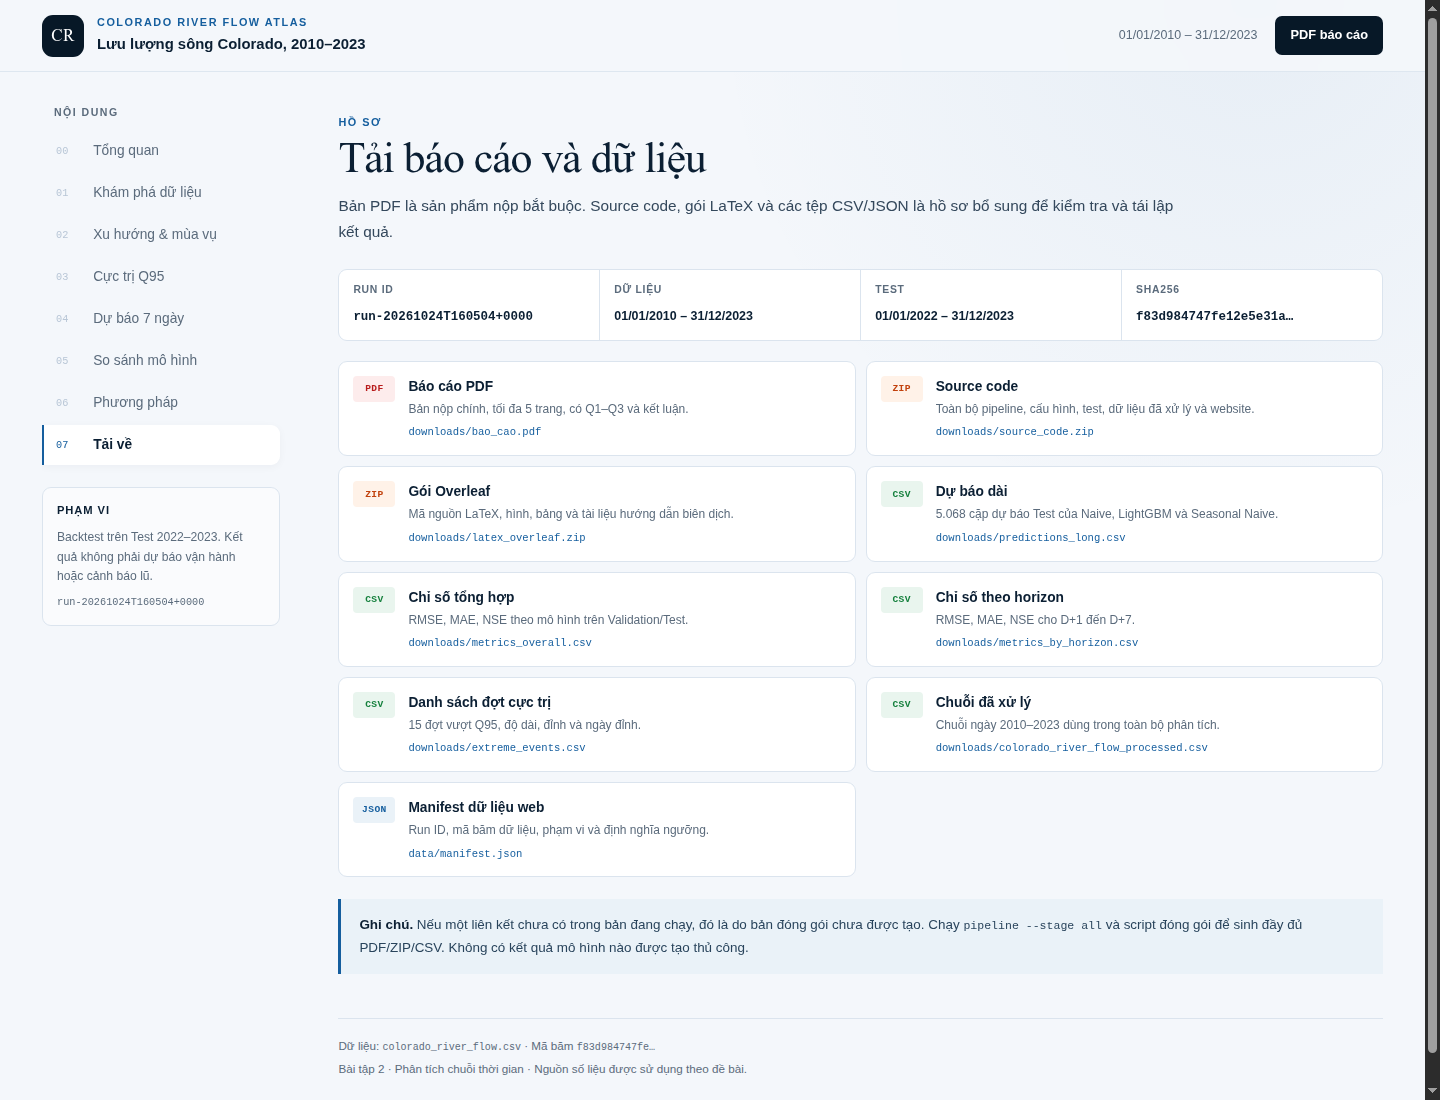
\includegraphics[width=0.94\linewidth]{website_downloads.png}
\caption{Trang Tải về với báo cáo, mã nguồn, dữ liệu và checksum.}
\label{fig:website-downloads}
\end{figure}

Việc công bố cả báo cáo, mã nguồn và dữ liệu giúp người đọc kiểm tra lại kết quả.
Tuy nhiên, cần phân biệt ba mức tái lập: (i) tái lập số liệu từ dữ liệu đã xử lý;
(ii) tái lập từ dữ liệu thô bằng pipeline; (iii) tái lập trong một môi trường phần
mềm khác. Báo cáo hỗ trợ mức (i) và (ii) thông qua script, manifest và seed; mức
(iii) phụ thuộc vào phiên bản thư viện và có thể thay đổi nhẹ do thuật toán tối ưu.

\subsection{Hiển thị trên thiết bị nhỏ}

Website được kiểm tra ở kích thước desktop và mobile. Hình~\ref{fig:website-mobile}
là ảnh chụp ở chiều rộng 375 px. Trên màn hình nhỏ, thanh điều hướng thu gọn, các
thẻ KPI xếp thành một cột và bảng có thể cuộn ngang. Mục tiêu không phải là tối ưu
cho mọi thiết bị mà là bảo đảm nội dung chính vẫn đọc được trên điện thoại.

\begin{figure}[H]
\centering
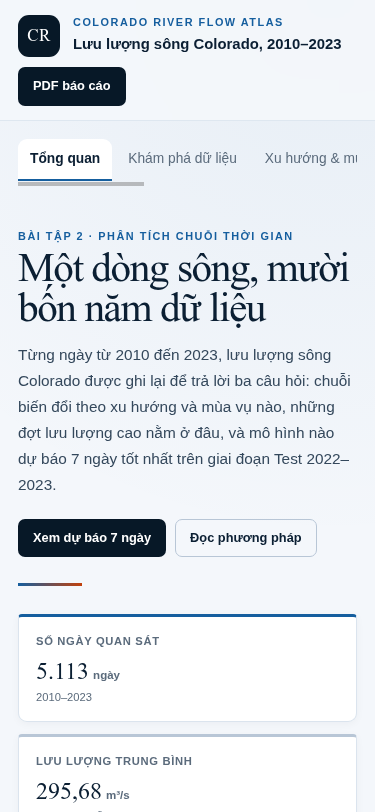
\includegraphics[width=0.28\linewidth]{website_mobile.png}
\caption{Website ở chiều rộng 375 px.}
\label{fig:website-mobile}
\end{figure}

\subsection{Triển khai và kiểm tra}

Website được triển khai tự động bằng GitHub Actions. Workflow chạy khi có push lên
\texttt{main}: cài dependency bằng \texttt{npm ci}, chạy \texttt{npm run build}, tải
thư mục \texttt{dist} lên GitHub Pages và deploy. Trong quá trình phát triển, workflow
đã chạy thành công; website công khai trả về HTTP 200. Các tệp PDF và source trong
trang Tải về đã được kiểm tra bằng mã băm so với bản local.

Một điểm cần lưu ý là GitHub Actions có thể hiển thị cảnh báo về phiên bản Node.js
của các action. Cảnh báo này không làm workflow thất bại trong lần chạy hiện tại,
nhưng cần được theo dõi khi GitHub thay đổi môi trường runner. Đây là vấn đề vận
hành, không ảnh hưởng đến nội dung khoa học của báo cáo.

\subsection{Giới hạn của website}

Website là kênh trình bày, không phải hệ thống cảnh báo. Nó không có backend, không
cập nhật dữ liệu thời gian thực và không đưa ra khuyến nghị vận hành. Các dự báo
được tính sẵn từ một lần chạy pipeline; nếu dữ liệu hoặc mô hình thay đổi, cần chạy
lại và deploy. Ngoài ra, website không thay thế báo cáo PDF: các lập luận, giới hạn
và trích dẫn đầy đủ nằm trong báo cáo, còn website tập trung vào tra cứu nhanh.
